

\section{Experiments}

We conducted various experiments to prove the effectiveness of the present method. 
Firstly, we qualitatively measure the results of our method on seen and unseen data, including action visualization and data downscaling visualization. 
Secondly, the generation quality and accuracy of action recognition were quantitatively measured for the six categories of target actions.
Finally, we performed comparison experiments with previous methods and ablation experiments with a special training loss term.
In addition, we train the ST-GCN using generated and real data, respectively, and test the accuracy of the same real data, thus evaluating the degree of approximation between the generated and real data. 

\subsection{Action Generation}

\textbf{Qualitative evaluation. }
Figure. \ref{fig:4} shows the generated seen actions. 
(a) and (b) are the “Reach into Pocket” and “Hopping” actions generated with reference to “Brush Hair”, respectively, the former being a hand motion and the latter a whole-body motion. 
(c) and (d) are the “Put Palms Together” and “Bow” actions generated with reference to “Hopping”, respectively. 
All the above actions preserve the source action $\textbf{M}_{src}$ category features and target action $\textbf{M}_{tgt}$ morphological features. 
Compared with Motion Puzzle, this method can generate hand, upper limb, and whole body actions without specifying body parts. 
Meanwhile, the temporal consistency of the actions is guaranteed, e.g., the real and generated “Hopping” are jumping at the same time in (b), and the bending tendency of the generated and real actions are consistent in (d). 

\begin{figure*}[htpb]
  \centering
   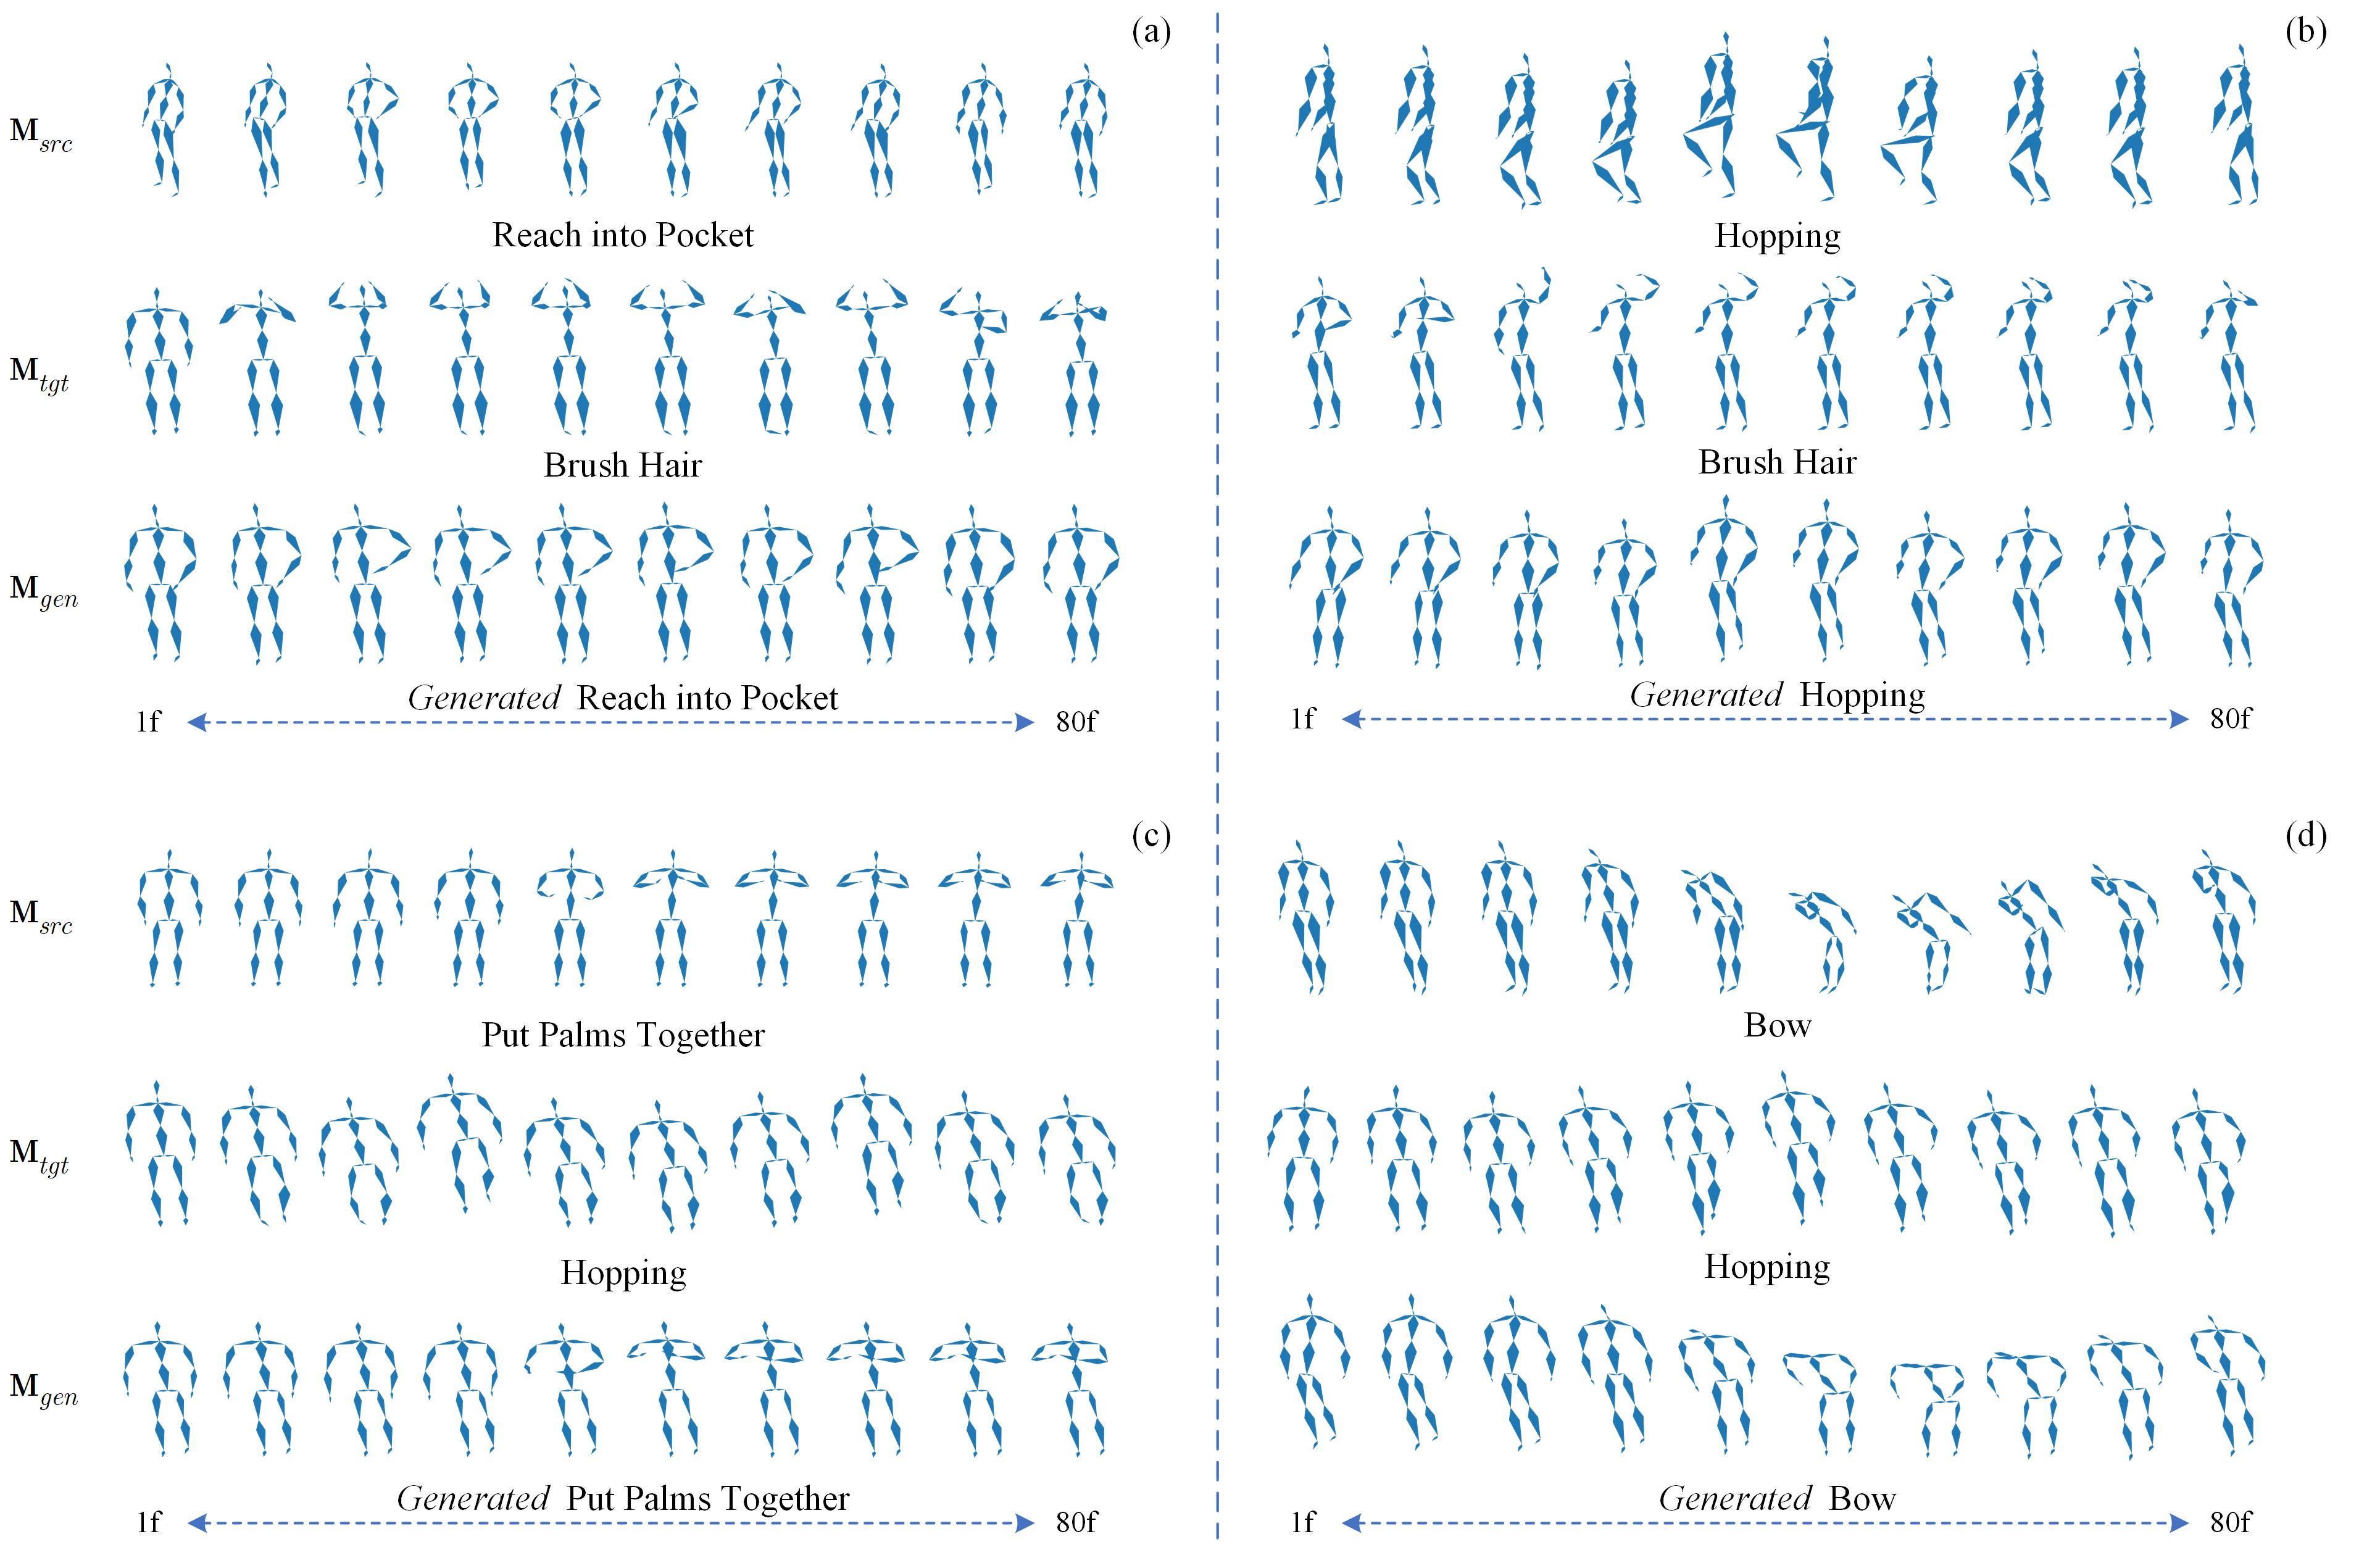
\includegraphics[width=0.75\linewidth]{figures/Fig4.jpg}

   \caption{Results generated by MGN on seen actions. (a) “Reach into Pocket”. (b) “Hopping”. (c) “Put Palms Together”. (d) “Bow”.}
   \label{fig:4}
\end{figure*}

Figure. \ref{fig:5} shows the generated unseen motions. 
It contains three cases: only the source action is unseen, only the target action is unseen, and both are unseen to thoroughly verify the transfer effect of unseen actions. 
In (a) and (f), the source action $\textbf{M}_{src}$  (“Drink Water” and “Jump Up”) is unseen, while the target action $\textbf{M}_{tgt}$  (“Kicking Something”) is seen. The generated action $\textbf{M}_{gen}$ can keep the category information of the source action. 
In (c) and (d), $\textbf{M}_{src}$  is seen, and $\textbf{M}_{tgt}$ is unseen. In $\textbf{M}_{gen}$, the morphological features of $\textbf{M}_{tgt}$ are transferred, and the “Kicking Something” action of $\textbf{M}_{src}$ is retained. 
Both source and target actions are unseen in (b) and (e). $\textbf{M}_{gen}$ shows that the model is still able to extract the category information of $\textbf{M}_{src}$ and the morphology information of $\textbf{M}_{tgt}$ to form a new action.
From the generated actions in Figure. \ref{fig:5}, our model can still generate high-quality actions that are unseen for the model.

\begin{figure*}[htpb]
  \centering
   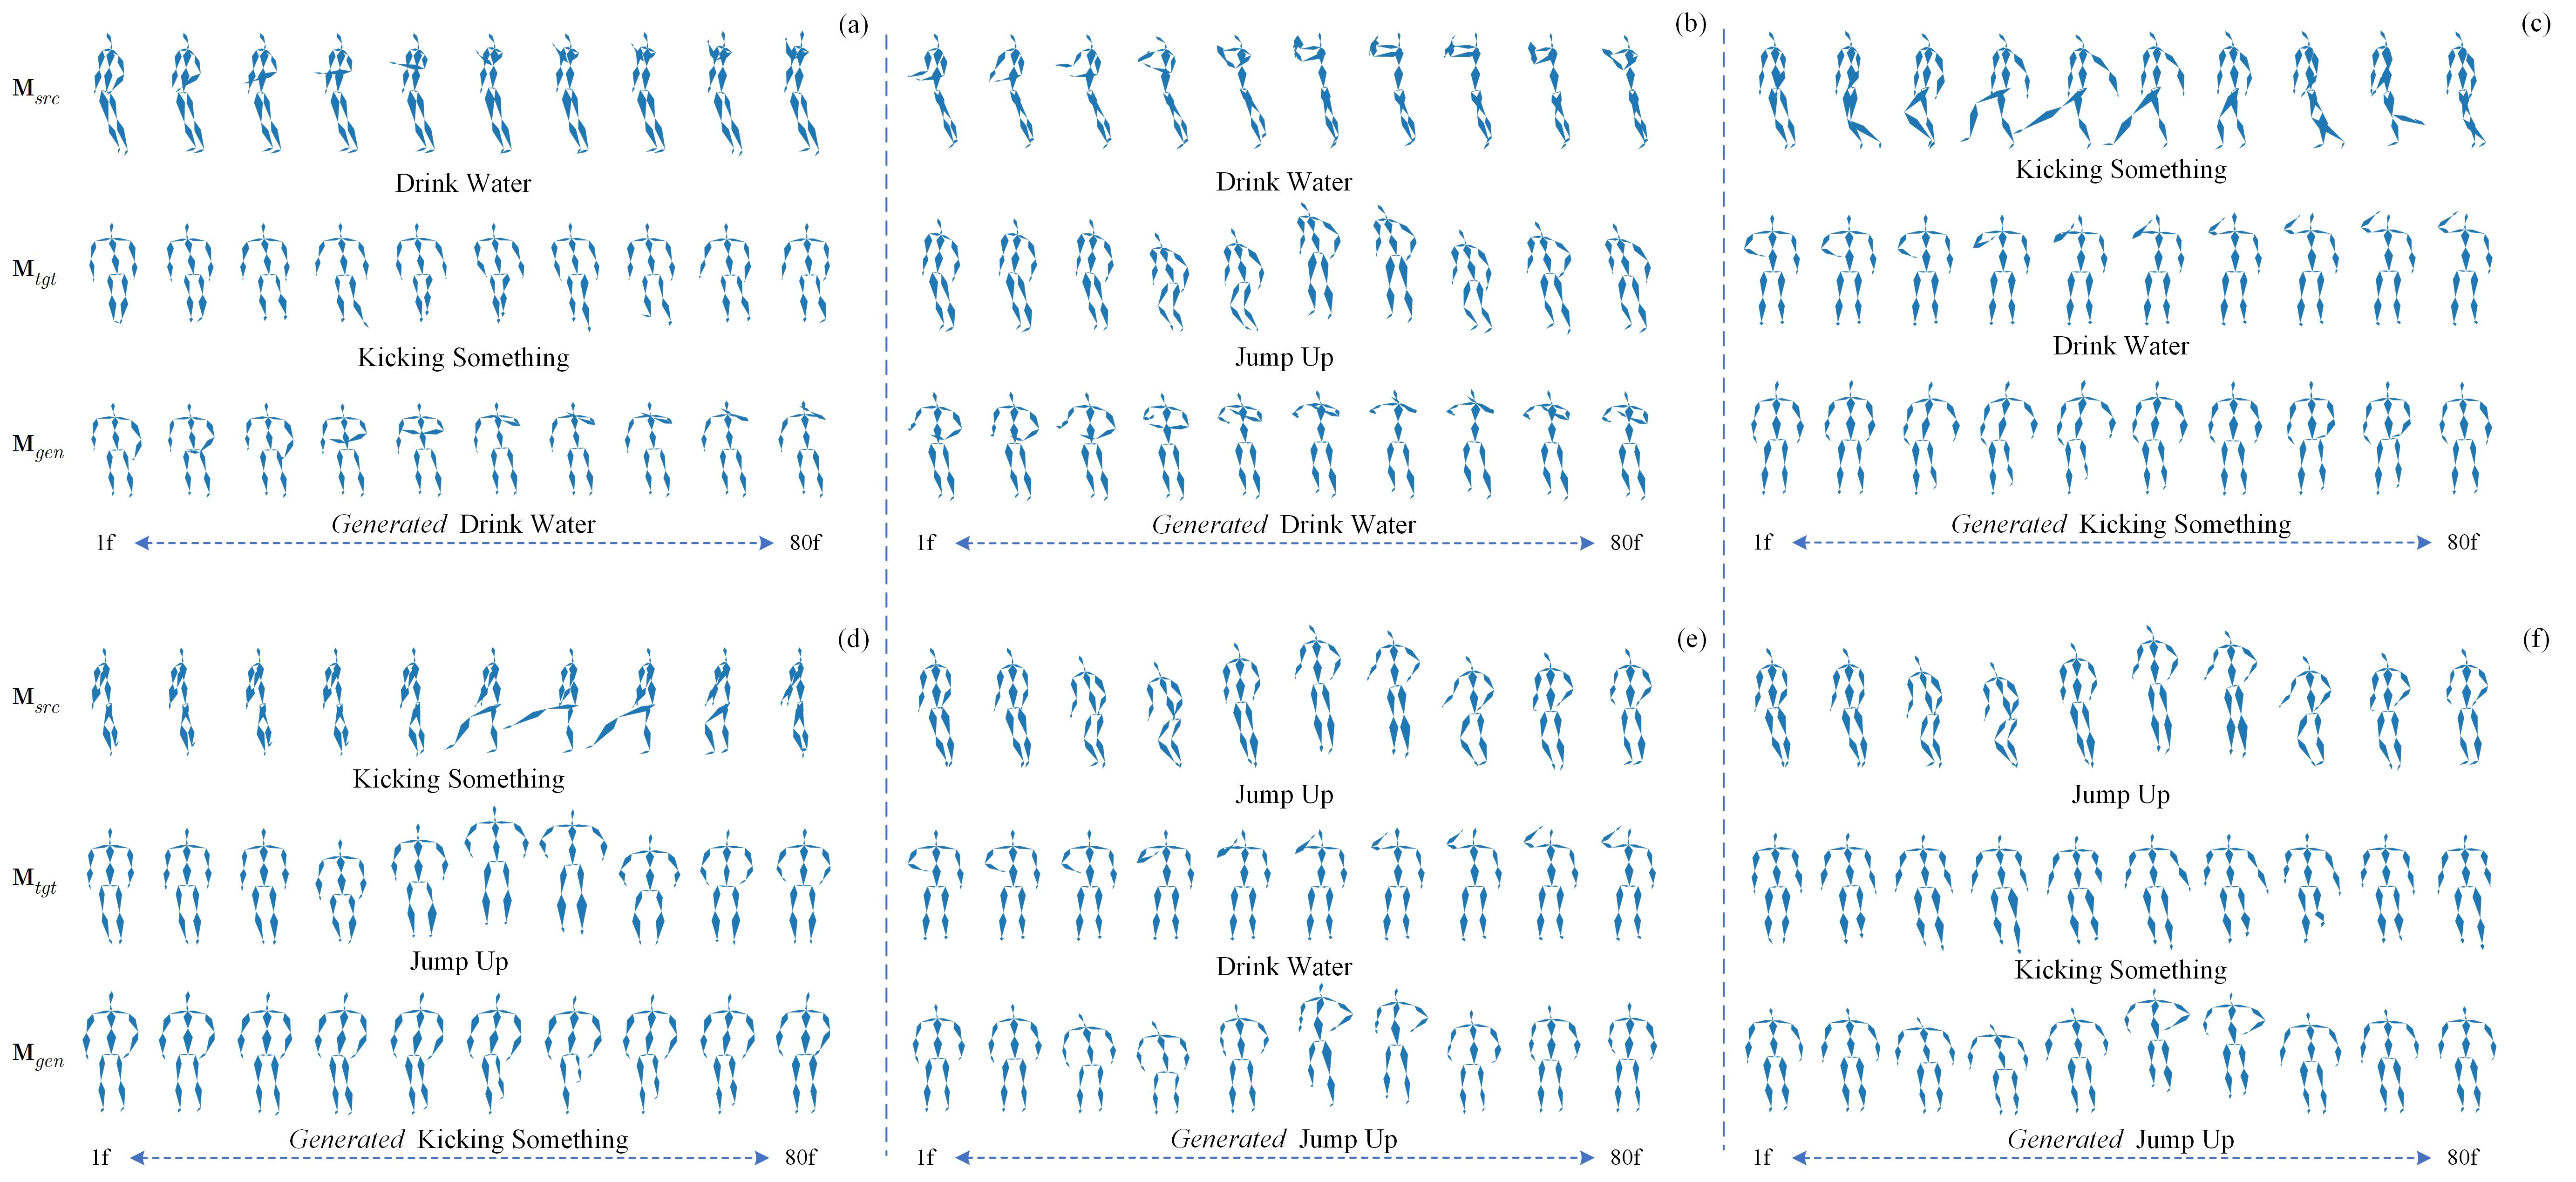
\includegraphics[width=\linewidth]{figures/Fig5.jpg}

   \caption{Results generated by MGN on unseen actions. (a) and (b) are  “Drink water” (Unseen). (c) and (d) are “Kicking Something” (Seen). (e) and (f) are “Jump Up” (Unseen).}
   \label{fig:5}
\end{figure*}

In order to verify the approximation between the generated data and the real data, t-SNE was used to visualize the action data. 
Figure. \ref{fig:3} shows the data distribution after dimensionality reduction using t-SNE. The black and red samples in the figure are the source actions, where red is a random sample in black. Cyan samples are the target actions, while green are the generated samples. The six figures show that the distribution of new actions generated using only one source action is similar to the distribution of source actions. The results show that our generated data can replace the original data. 

\begin{figure*}[htpb]
  \centering
   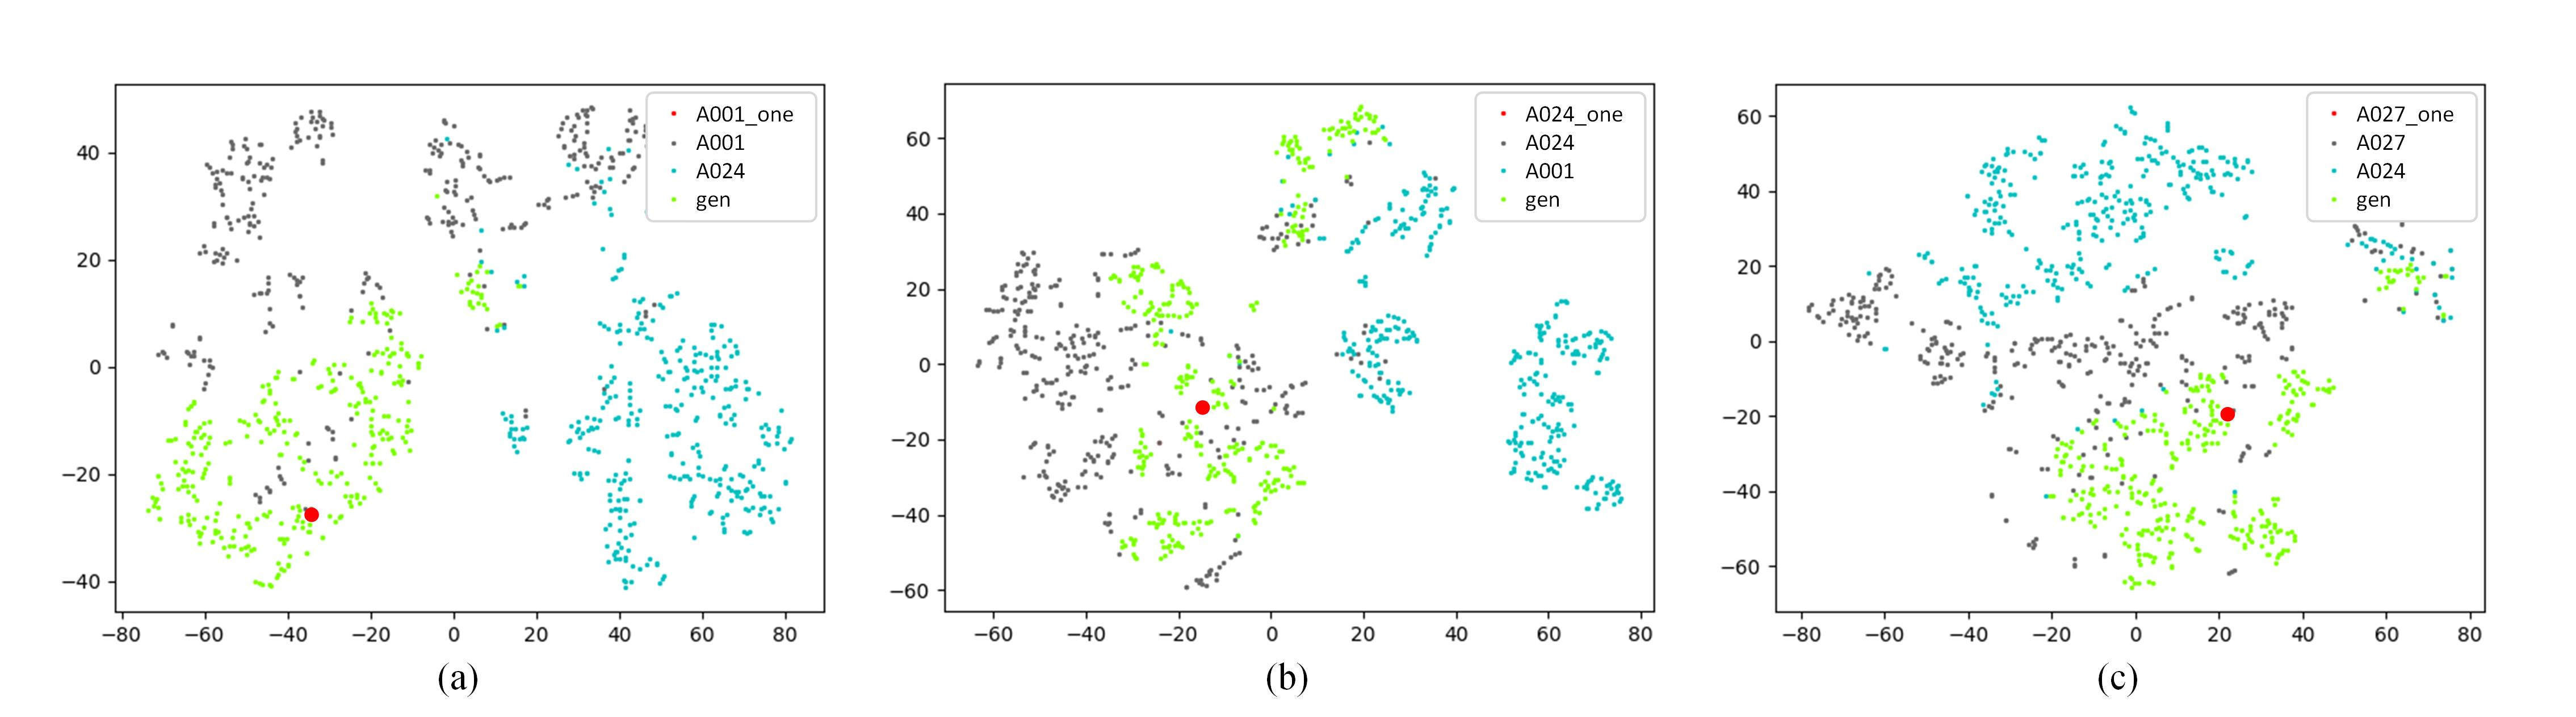
\includegraphics[width=0.8\linewidth]{figures/Fig3.jpg}

   \caption{Action data is projected into 2D space using t-SNE, where black is the source action, red is a sample of black, cyan is the target action, and green is some new action generated using a sample of red and some cyan. The green sample and the black sample are very close to each other in space, which indicates that the generated actions conform to some extent to the distribution of the source actions.}
   \label{fig:3}
\end{figure*}

\textbf{Quantitative evaluation. }
We quantitatively measured the quality of generation and accuracy of action recognition on seen and unseen data. 
Specifically, we use two metrics: Fréchet Motion Distance (FMD) and Accuracy (Acc). 
We compute FMD and Acc on the action set based on all possible combinations of source and target actions generated by the MGN.

The FMD measures the similarity between the feature vectors of real and generated actions, similar to the Fréchet Inception Distance (FID). 
The action classifier is trained by the ST-GCN method, and feature vectors are obtained after the maximum pooling layer to compute the FMD of generated and real actions. 
A lower FMD means a higher quality of action.

% As described in Sec. \ref{sec:Dataset}, 
We complete the experimental evaluation using the action sets $\mathcal{M}_{full}$, $\mathcal{M}_{seen}$, and $\mathcal{M}_{unseen}$. 
The $\mathcal{M}_{seen}$ contains six categories of seen actions data: “Brush Teeth”, “Pick up”, “Reading”, “Take off a Hat”, “Kicking Something”, and “Sneeze”, for 3996 samples. 
The $\mathcal{M}_{unseen}$ contains six categories of unseen actions data: “Drink Water”, “Throw”, “Sit Down”, “Clapping”, “Jump up”, and “Bow”, for 3992 samples.
Table \ref{tab:1} shows that the Acc of the generated actions all exceeded 90\%. 
The highest of these is 95.39\%, with an average of 92.18\% under the seen actions data. 
The highest of these is 97.20\%, with an average of 94.42\% under the unseen actions data. 
The mean values of FMD in both cases are 2.11 and 2.67, respectively. This shows that our generated actions are high-quality and can be well recognized by the action classifier. 

\begin{table}
  \centering
  % \begin{tabular}{@{}lc@{}}
  \resizebox{1\columnwidth}{!}{
  \begin{tabular}{cccccccc}
    \toprule
    \multirow{2}*{}&\multirow{2}*{Metric}&\multicolumn{6}{c}{Target motion}\\
\cline{3-8}
    &  &  A0&  A1&  A2&  A3&  A4& A5\\
    \midrule
    \multirow{2}*{Seen}& Acc(\%)&  91.10&  90.12&  94.63&  92.29&  95.39& 89.54\\  
    & FMD &  2.19&  2.00&  1.95&  2.02&  2.18& 2.31\\ 
    \multirow{2}*{Unseen}& Acc(\%)&  97.20&  96.45&  89.62&  90.78&  96.77& 95.72\\
    & FMD &  3.21&  2.49&  2.53&  3.11&  2.30& 2.35\\
    \bottomrule
  \end{tabular}}
  \caption{Quantitative evaluation. We calculated FMD and Acc using $\mathcal{M}_{full}$, $\mathcal{M}_{seen}$, and $\mathcal{M}_{unseen}$. $\mathcal{M}_{full}$ contains six categories of action: “Brush Hair”, “Writing”, “Put on a Shoe”, “Take off Glasses”, “Hopping”, and “Shake Head”. For representation simplicity, we numbered the six categories of target action as A0, A1, A2, A3, A4, and A5.}
  \label{tab:1}
\end{table}

\subsection{Action Recognition}
\label{sec:motion recognition}

Generating compelling and high-quality data is significant for action recognition tasks when specific action categories are scarce. 
In order to measure the degree of similarity between generated and real data fully, an action recognition model is trained using generated and real actions, respectively. 

We divided the actions in $\mathcal{M}_{unseen}$ into a training set $\mathcal{M}_{\hat{train}}$ and a test set $\mathcal{M}_{\hat{test}}$. An action recognition model (ST-GCN) is trained using $\mathcal{M}_{\hat{train}}$ and tested on $\mathcal{M}_{\hat{test}}$. As shown in the Table \ref{tab:2}, the top-1 accuracy is 91.80\%.  
We sample one-shot and few-shot (1\%, 5\%, and 10\%) from $\mathcal{M}_{\hat{train}}$ for action generation. 
Subsequently, the generated and sampled actions are concatenated into a new train set to train and test the ST-GCN. 
As shown in Table \ref{tab:2}, the top-1 accuracy is highest at 91.62\% when sampling 10\%, which is only 0.18\% lower than that of $\mathcal{M}_{\hat{train}}$. When sampling 1\% and 5\%, the top-1 accuracy is still high, close to 90\%. 
However, the top-1 accuracy is lower when sampling one, with a maximum of only 62.84\%. 
This result is expected because when sampling a single sample, the generative model is very limited to learning the source data distribution, leading to a large deviation of the generated data distribution from the original complete data distribution. 

\begin{table}
  \centering
  % \begin{tabular}{@{}lc@{}}
  \resizebox{1\columnwidth}{!}{
  \begin{tabular}{cccccc}
    \toprule
    \multirow{2}*{Target motion}&\multirow{2}*{OneShot(\%)}& \multicolumn{3}{c}{FewShot(\%)} & \multirow{2}*{$\mathcal{M}_{\hat{train}}$(\%)}\\ \cline{3-5} 
        && 1\% & 5\% & 10\% &\\
    \midrule
    A0 & 62.84 & 84.09 & 88.34 & 91.62 & \multirow{6}*{91.80} \\ 
    A1 & 53.31& 79.54 & 89.74 & 90.04 &  \\  
    A2 & 57.62 &  78.14& 89.01 & 91.32 & \\ 
    A3 & 57.07& 81.30& 89.25 & 91.44 & \\
    A4 & 45.96& 82.33 & 88.16& 91.14 & \\
    A5 & 61.57 & 83.49 & 88.46 & 91.01 & \\
    \bottomrule
  \end{tabular}}
  \caption{Top-1 accuracy comparison. Sampling one-shot and few-shot (1\%, 5\%, and 10\%) from $\mathcal{M}_{\hat{train}}$ for action generation. The generated and sampled actions are concatenated into a new train set to train and test the ST-GCN. }
  \label{tab:2}
\end{table}

\subsection{Ablation Study and Comparison with Prior Work}

We conduct an ablation study of the loss term and a comparison with other methods to verify the validity of the loss term in the model and the state-of-the-art of our method. 
Specifically, we quantitatively measure the generation quality and Accuracy of the five generative models: 
$[$Aberman et al. 2020$]$, 
$[$Jang et al. 2022$]$, 
MGN($\mathcal{L}_{rec}+\mathcal{L}_{cyc}$), 
MGN($\mathcal{L}_{rec}+\mathcal{L}_{cyc}+\mathcal{L}_{trip}$), and AGN (Table. \ref{tab:3}).
Where MGN($\mathcal{L}_{rec}+\mathcal{L}_{cyc}+\mathcal{L}_{trip}$) is a part of AGN. Therefore, the FMD is both 2.67. 
Due to the effect of UMN, the recognition accuracy of AGN is 4.76\% higher than the former, which is 87.42\% and 92.18\%, respectively. 
The FMD and Accuracy are 2.90 and 83.43\% for the MGN without $\mathcal{L}_{trip}$, proving that our design of $\mathcal{L}_{trip}$ is effective in generative networks. The method of Aberman et al. measures the FMD to be 21.36 and the Accuracy to be 51.34\%. Motion Puzzle measured an FMD of 9.42 and an Accuracy of 67.63\%.
In comparison, our method is competitive.

\begin{table}
  \centering
  % \begin{tabular}{@{}lc@{}}
  \resizebox{1\columnwidth}{!}{
  \begin{tabular}{lcc}
    \toprule
    Methods&FMD$\downarrow$&Acc(\%)$\uparrow$ \\
    \midrule
    $[$Aberman et al. 2020$]$& 21.36 $\pm$ 2.37& 51.34 $\pm$ 1.92\\
    $[$Jang et al. 2022$]$& 9.42 $\pm$ 0.72& 67.63 $\pm$ 3.95 \\
    \midrule
    MGN ($\mathcal{L}_{rec}+\mathcal{L}_{cyc}$) & 2.90 $\pm$ 0.54& 83.43 $\pm$ 3.21 \\ 
    MGN ($\mathcal{L}_{rec}+\mathcal{L}_{cyc}+\mathcal{L}_{trip}$) & 2.67 $\pm$ 0.37& 87.42 $\pm$ 2.24 \\
    \textbf{AGN (Ours)}& \textbf{2.67 $\pm$ 0.37}& \textbf{92.18 $\pm$ 2.75} \\
    \bottomrule
  \end{tabular}}
  \caption{FMD and Acc are measured using five methods: [Aberman et al. 2020], [Jang et al. 2022], MGN($\mathcal{L}_{rec}+\mathcal{L}_{cyc}$), MGN($\mathcal{L}_{rec}+\mathcal{L}_{cyc}+\mathcal{L}_{trip}$), and AGN.}
  \label{tab:3}
\end{table}

\begin{figure*}[htpb]
  \centering
   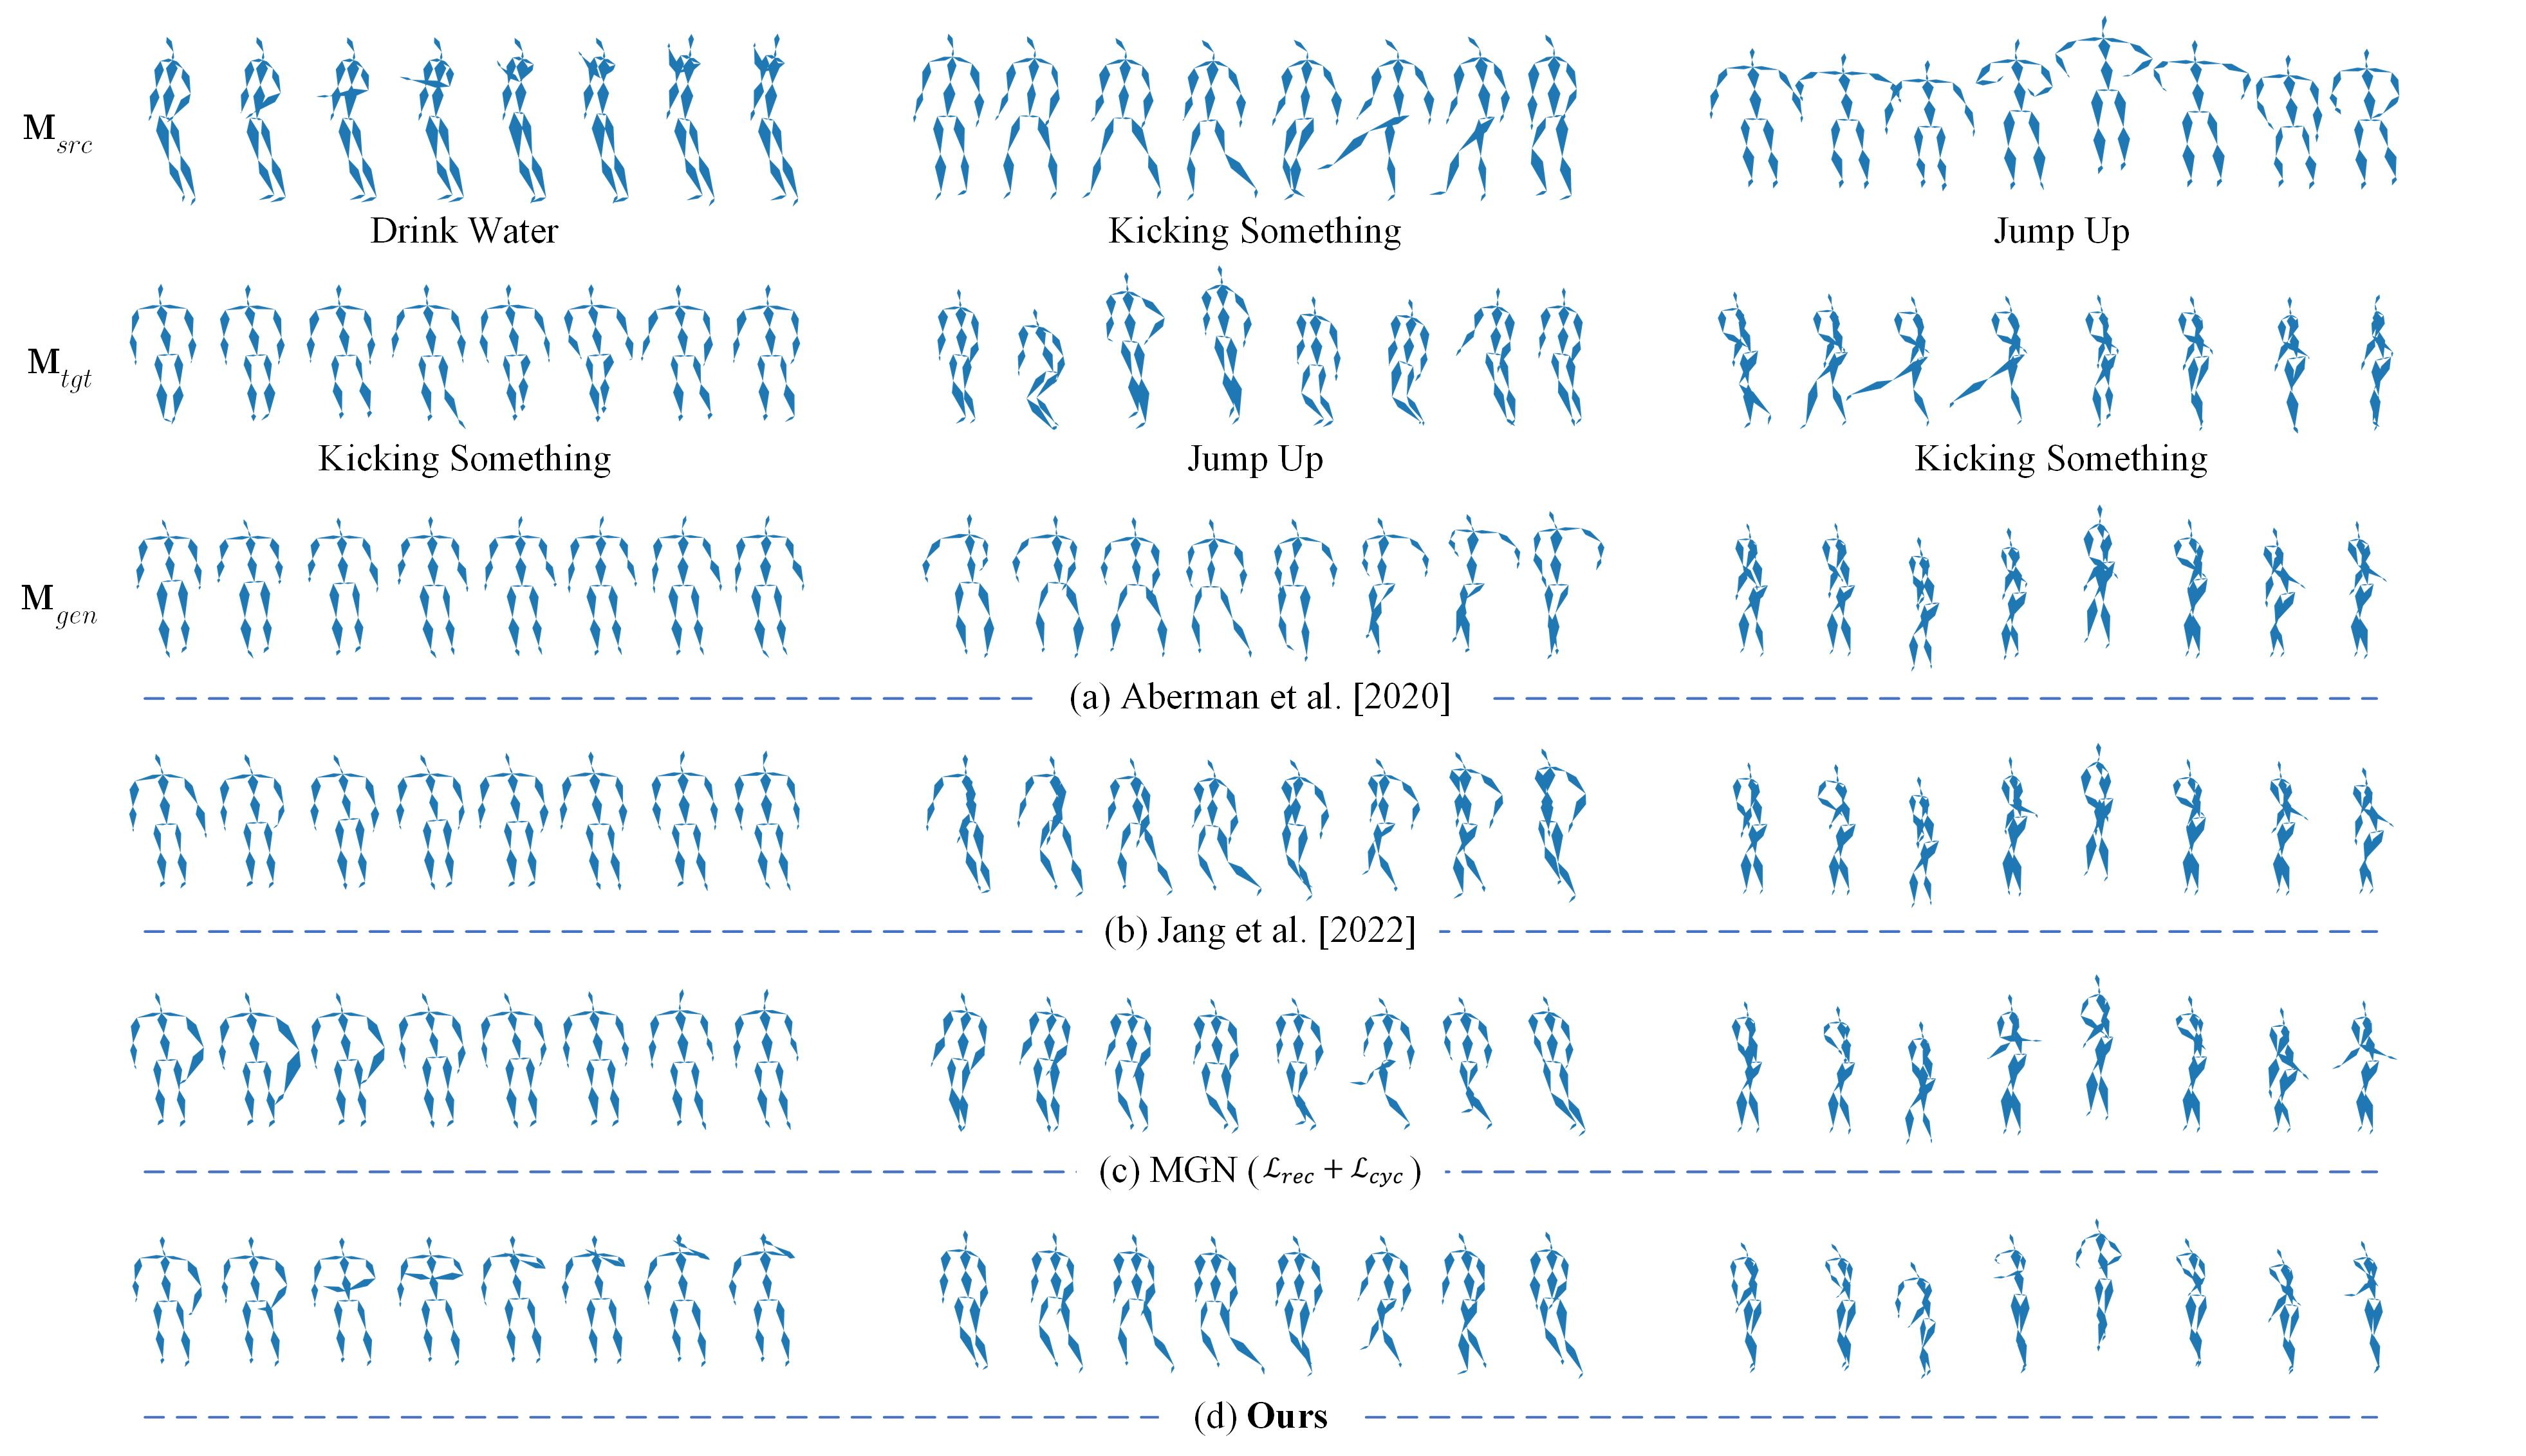
\includegraphics[width=0.8\linewidth]{figures/Fig6.jpg}

   \caption{Comparison results. We used four methods to generate hand action (“Drinking Water”), leg action (“Kicking Something”), and whole-body action (“Jump up”).}
   \label{fig:6}
\end{figure*}

Figure. \ref{fig:6} shows the actions generated by the four methods: (a) the actions generated by Aberman's method, (b) the actions generated by Motion Puzzle, (c) the actions generated by MGN ($\mathcal{L}_{trip}$), and (d) the actions generated by our method.  
Compared to other methods, our method is optimal in generating hand action (“Drinking Water”), leg action (“Kicking Something”), and whole-body action (“Jump up”). 
In (a), (b), and (c), the “Drink Water” (first column) contains only the body morphology of the target action but not the hand moves of the source action. 
The “kicking Something” (second column) and “Jump up” (third column) combine the category features of the source action and the morphology features of the target action very well, but the hand moves are very raw.
Our method generates more natural and coordinated actions, both in terms of the moves of the parts and the overall morphology.

To fully demonstrate that UMN is effective, we sampled 1\% from $\mathcal{M}_{\hat{train}}$ and generated actions using MGN and MGN+UMN, respectively. Then, it is tested according to the action recognition experiment (sec. \ref{sec:motion recognition}). 
Table \ref{tab:4} shows that the average recognition accuracy is 81.48\% for MGN+UMN and 64.96\% for MGN. The results demonstrate that the UMN is effective.

\begin{table}
  \centering
  % \begin{tabular}{@{}lc@{}}
  \resizebox{1\columnwidth}{!}{
  \begin{tabular}{lcccccc}
    \toprule
    & A0 &  A1 & A2 & A3 & A4 & A5  \\
    \midrule
    MGN($\mathcal{L}_{total}$)& 58.29 & 62.72 & 74.62 & 57.32 & 67.88 & 68.91 \\
    MGN($\mathcal{L}_{total}$)+UMN& 84.09 & 79.54 & 78.14 & 81.30 & 82.33 & 83.49 \\
    \bottomrule
  \end{tabular}}
  \caption{Comparison of Top-1 accuracy of MGN($\mathcal{L}_{total}$) and MGN($\mathcal{L}_{total}$)+UMN. Sampling 1\% from $\mathcal{M}_{\hat{train}}$ for action generation.}
  \label{tab:4}
\end{table}
